This section describes the numerical optimization approach for
calculating bounds on mortality within arbitrary percentiles of the
education distribution. To calculate bounds, we discretize the mortality-education relationship and solve a numerical optimization problem that obtains the highest and lowest possible values of expected mortality at any given point, that are consistent with matching the empirical data points and meeting a set of structural constraints on the functional form of the CEF. We first formalize the computational procedure and then describe its numerical implementation.

\subsubsection{Conceptual Approach: Functions of the CEF} 
We write the conditional expectation function in the form
$Y(x) = s(x,\gamma)$, where $\gamma$ is a finite-dimensional vector
that lies in parameter space $G$ and serves to parameterize the CEF
through the function $s$. For example, we could estimate the
parameters of a linear approximation to the CEF by defining
$s(x,\gamma)=\gamma_0+\gamma_1*x$. We can approximate an arbitrary
nonparametric CEF by defining $\gamma$ as a vector of discrete values
that give the value of the CEF in each of $N$ partitions; we take this
approach in our numerical optimizations, setting $N$ to
100.\footnote{For example, $s(x,\gamma_{50})$ would represent $E(y|x
  \in [49,50])$.} Any statistic $m$ that is a single-valued function
of the CEF, such as the average value of the CEF in an interval
$(\mu_a^b)$, or the slope of the best fit line to the CEF, can be
defined as $m(\gamma)=M(s(x,\gamma))$.

Let $f(x)$ represent the probability distribution of $x$. Define $\Gamma$ as the set of parameterizations of the CEF that obey monotonicity and minimize mean squared error with respect to the observed interval data:
\begin{align}
  \label{eq:opt1}
  \Gamma = \underset{g \in G}{\text{argmin}} \sum_{k=1}^K \Bigg\{
  \int_{x_k}^{x_{k+1}} f(x) dx \left( \left(
  \frac{1}{\int_{x_k}^{x_{k+1}} f(x)dx } \int_{x_k}^{x_{k+1}} s(x,g)
  f(x) dx \right) - \overline{r}_k \right)^2 \Bigg\} \\ \nonumber
  \text{such that} \\ \tag{Monotonicity} s(x,g) \text{ is weakly
    increasing in } x.
\end{align}
\noindent Decomposing this expression, $\frac{1}{\int_{x_k}^{x_{k+1}}
  f(x)dx } \int_{x_k}^{x_{k+1}} s(x,g) f(x) dx$ is the mean value of
$s(x,g)$ in bin $k$, and $\int_{x_k}^{x_{k+1}} f(x) dx$ is the mass in
bin $k$. The minimand is thus a bin-weighted MSE.\footnote{While we
  choose to use a weighted mean squared error penalty, in principle
  $\Gamma$ could use other penalties.} Recall that for the rank
distribution, $x_1=0$ and $x_{K+1}=100$. We can easily add additional
structural constraints on $s(x,\gamma)$ to Equation \ref{eq:opt1} (e.g., the curvature
constraint below) or remove the monotonicity constraint. 

The bounds on $m(\gamma)$ are therefore:

\begin{equation}
  \begin{aligned}
    \label{eq:m_bounds}
    m^{min} &= \inf\{m(\gamma) \ \vert \ \gamma \in \Gamma \} \\ m^{max} &= \sup\{m(\gamma) \ \vert \ \gamma \in \Gamma \}.
  \end{aligned}
\end{equation}

For example, bounds on the best linear approximation to the CEF can be defined by the following process. First, consider the set of all CEFs that satisfy monotonicity and minimize mean-squared error with respect to the observed bin means.\footnote{In many cases, and in all of our applications, there will exist many such CEFs that exactly match the observed data and the minimum mean-squared error will be zero.} Next, compute the slope of the best linear approximation to each CEF. The largest and smallest slope constitute $m^{min}$ and $m^{max}$. Note that this definition of the best linear approximator to the CEF corresponds to the \textit{least squares set} defined by \citet{Ponomareva2011}.

The set of CEFs that describe the upper and lower bounds in Proposition~\ref{eq:cef_bound} are step functions with substantial discontinuities. If such functions are implausible descriptions of the data, then the researcher may wish to impose an additional constraint on the curvature of the CEF, which will generate tighter bounds. For example, examination of the mortality-income relationship (which can be estimated at each of 100 income ranks, displayed in Appendix Figure \ref{fig:mort_poly}) suggests no such discontinuities. Alternately, in a context where continuity has a strong theoretical underpinning but monotonicity does not, a curvature constraint can substitute for a monotonicity constraint and in many cases deliver useful bounds.

We consider a curvature restriction with the following structure:
\begin{align}
  \label{eq:c_bar}
  \tag{Curvature Constraint} \tag{Or alt Curvature} s(x,\gamma) \text{ is twice-differentiable and } \vert s''(x,\gamma) \vert \leq \overline{C}.
\end{align}

\noindent This is analogous to imposing that the first derivative is Lipshitz.\footnote{Let $X, Y$ be metric spaces with metrics $d_X, d_Y$ respectively. The function $f:X \to Y$ is \textit{Lipschitz continuous} if there exists $K \geq 0$ such that for all $x_1,x_2 \in X$,
  $$d_Y(f(x_1),f(x_2)) \leq K d_X(x_1,x_2).$$} Depending on the value
of $\overline{C}$, this constraint may or may not bind. 

The most restrictive curvature constraint, $\overline{C}=0$, is
analogous to the assumption that the CEF is linear. Note that the
default practice in many studies of mortality is to estimate the best
linear approximation to the CEF of mortality given education (e.g.,
\citet{Cutler2011} and \citet{Goldring2016}). A moderate curvature
constraint is therefore a \textit{less} restrictive assumption than
the approach taken in many studies. In practice, we slightly adjust the curvature
constraint condition by generating a ``normalized'' curvature
constraint which imposes that the absolute value of the second
derivative, divided by the mean mortality across all percentiles, does
not exceed a certain $\overline{C}$. The advantage of this approach is
that it more readily permits using a conservative value of $\overline{C}$ across
all groups. We discuss the choice of curvature
restriction below. 

\subsubsection{Computational Approach} 

This section describes a method to numerically solve the constrained optimization problem suggested by Equations~\ref{eq:opt1} and \ref{eq:m_bounds}. 

To make the problem numerically tractable, we solve the discrete problem of identifying the feasible mean value taken by $E(y|x)$ in each of $N$ discrete partitions of $x$. We thus assume $E(y|x) = s(x,\gamma)$, where $\gamma$ is a vector that defines the mean value of the CEF in each of the $N$ partitions. We use $N=100$ in our analysis, corresponding to integer rank bins, but other values may be useful depending on the application. In other words, we will numerically calculate upper and lower bounds on $E(y|x \in [0, 1])$, $E(y|x \in [1, 2])$, $...$, $E(y|x \in [99,100])$.  Given continuity in the latent function, the discretized CEF will be a very close approximation of the continuous CEF; in our applications, increasing the value of $N$ increases computation time but does not change any of our results.

We solve the problem through a two-step process. Define a $N$-valued
vector $\hat{\gamma}$ as a candidate CEF. First, we calculate the
minimum MSE from the constrained optimization problem given by
Equation~\ref{eq:opt1}. Put another way, each set $\Gamma$
  is associated to a minimmum MSE (the value of the objective), which
  we denote $\underbar{MSE}$. We then run a second pair of constrained optimization problems that respectively minimize and maximize the value of $m(\hat{\gamma})$, with the additional constraint that the MSE is equal to the value obtained in the first step, denoted $\underbar{MSE}$. Equation \ref{eq:opt2} shows the second stage setup to calculate the lower bound on $m(\hat{\gamma})$:
\begin{align}
  \label{eq:opt2}
  m^{min} &= \underset{ \hat{\gamma} \in [0,100]^{N} }{ \text{min} } m(\hat{\gamma}) \\
  &\nonumber \text{such that} \\
  \tag{Monotonicity} s(x, \hat{\gamma}) \text{ is weakly increasing in } x \\
  \tag{Curvature} \lvert s''(x, \hat{\gamma}) \rvert &\leq \overline{C} \\
  \tag{MSE Minimization} \sum_{k=1}^K \left[ \frac{\Vert X_k \Vert}{100} \left( \left( \frac{1}{\Vert X_k \Vert} \sum_{x \in X_k} s(x,\hat{\gamma}) \right) - \overline{r}_k \right)^2 \right] &= \underbar{MSE}
\end{align}

\noindent
$X_k$ is the set of discrete values of $x$ between $x_{k}$ and
$x_{k+1}$ and $\Vert X_k \Vert$ is the width of bin
$k$. $\overline{r}_k$ is the observed mortality in education bin $k$,
and \underbar{MSE} is the lowest mean-squared error obtainable out of
the entire set of education-mortality functions, which is typically
zero. The complementary maximization problem obtains the upper bound
on $m(\hat{\gamma})$. Note that this particular setup is specific to
the uniform rank distribution, but setups with other distributions
would be similar. 

The purpose of the two-step process is that it is difficult to
numerically solve for every possible member of $\Gamma$ under
arbitrary constraints. We render the problem tractable by recasting
the problem as a minimization problem of obtaining $\underbar{MSE}$ in
the first step. Then, in the second step, we use $\underbar{MSE}$ as a
constraint. 

Note that setting $m(\gamma) = \gamma_x$ (the $x$\superscript{th} element of $\gamma$) obtains bounds on the value of the CEF at point $x$. Calculating this for all ranks $x$ from 1 to 100 generates analogous bounds to those derived in proposition \ref{eq:cef_bound}, but satisfying the additional curvature constraint. Similarly $m(\gamma) = \frac{1}{b-a} \sum_{x=a}^{b}\gamma_x$ yields bounds on $\mu_a^b$.

The numerical method can easily permit the curvature constraint to vary over the CEF. For example, one might believe that there are discontinuities in the CEF at bin boundaries, due to sheepskin effects \citep{hungerford1987}; high-school graduates, upon receiving a diploma, could experience discretely lower mortality probability due to better labor-market outcomes. In other settings, researchers might impose that the CEF has a large (but finite) curvature in one portion of its domain and be more constrained elsewhere.

\textbf{Calibrating a curvature constraint}.  This subsection explains how we obtain a benchmark for the curvature constraint using data from \citet{Chetty2016b} on mortality rates for U.S. men and women above age 40 from years 2001--2014. We collapse the data to three-year periods and five-year age groups.\footnote{Since the number of years is not divisible by 3, we group years 2001 and 2002.}$^,$\footnote{Because people are ranked within the percentile for their own age, gender, and year, this departs slightly from the ranking procedure we use in the text.} We then use OLS to fit fifth-order polynomials to the mortality-income percentile data we observe. We show two examples of these best-fit functions for 50--54 year old men and women in 2012--2014 (the last year data are available), as well as the range for the normalized second derivative for these groups, in Appendix Figure \ref{fig:mort_poly}. The $\overline{C}$ we use is 50\% larger than the maximum absolute value of the union of these ranges across all such groups we observe.

We construct a $\overline{C}$ that holds for all mortality-income
functions as follows. Using the estimated polynomial fit, we
analytically compute the absolute value of the second derivative of
the best-fit polynomial at every value for every polynomial
function. To generate comparable $\overline{C}$, we construct a normalized $\overline{C}$ that accounts for differences in mortality levels by dividing the absolute value of the second derivative by the mean mortality in that age-year group (across all percentiles). Expressed in these terms (and multiplied by 100), the normalized $\overline{C}$ represents the absolute value of the second derivative as a percent of the mean.

Across all age and years, the largest $\overline{C}$ is approximately 2.0\%. Because polynomial fits can be inaccurate near the tails, we also compute the largest second-derivative (normalized by the mean mortality across all percentiles) within the set of percentiles $[5,95]$. This value is 1.5\%. We choose a conservative curvature constraint of 3\% --- about 50\% larger than the largest normalized $\overline{C}$ observed in the data.

We acknowledge the concern that mortality-income CEFs may exhibit different curvature than mortality-education CEFs. We argue that the mortality-income CEF at least provides a natural benchmark for how curved the CEF might be in the education setting; we are not aware of another continuous conditioning value to calibrate $\overline{C}$. Moreover, we are comforted that our results are robust to relaxing the curvature constraint altogether.

%%%%%%%%%%%%%%%%%%%%%%%%%%%%%%%%
% Mortality rank distributions 
%%%%%%%%%%%%%%%%%%%%%%%%%%%%%%%%
\begin{figure}[H]
  \caption{Fifth-Order Polynomial Approximations to the Empirical Mortality-Income CEF}
  \label{fig:mort_poly}

\begin{center}
  Panel A: 50--54 Year-Old Women in 2012--2014
\end{center}
  \begin{center}
      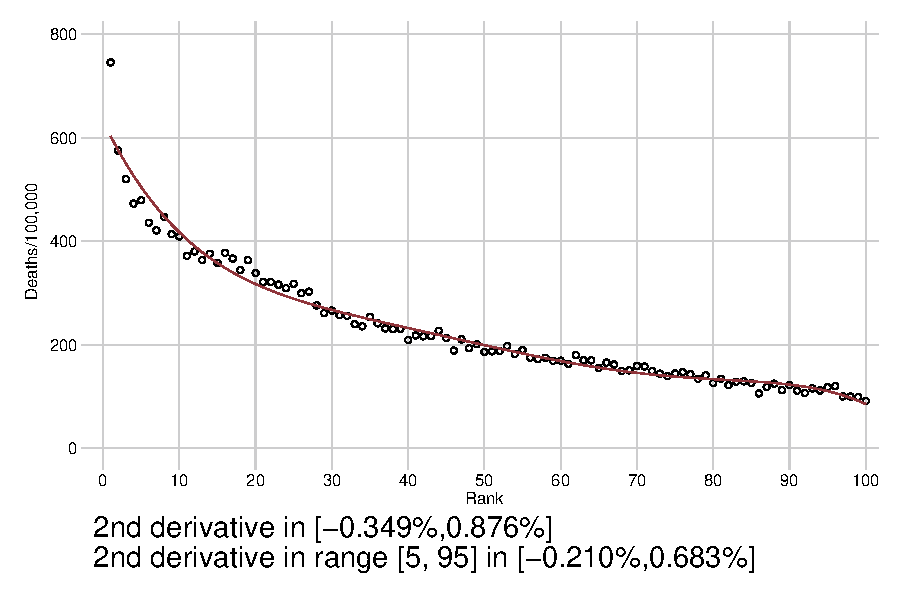
\includegraphics[scale=0.75]{\mortalitypath/polyspline__50_F_2012-2014}
  \end{center}

\begin{center}  
  Panel B: 50--54 Year-Old Men in 2012--2014 
\end{center}
  \begin{center}                                                          %%
      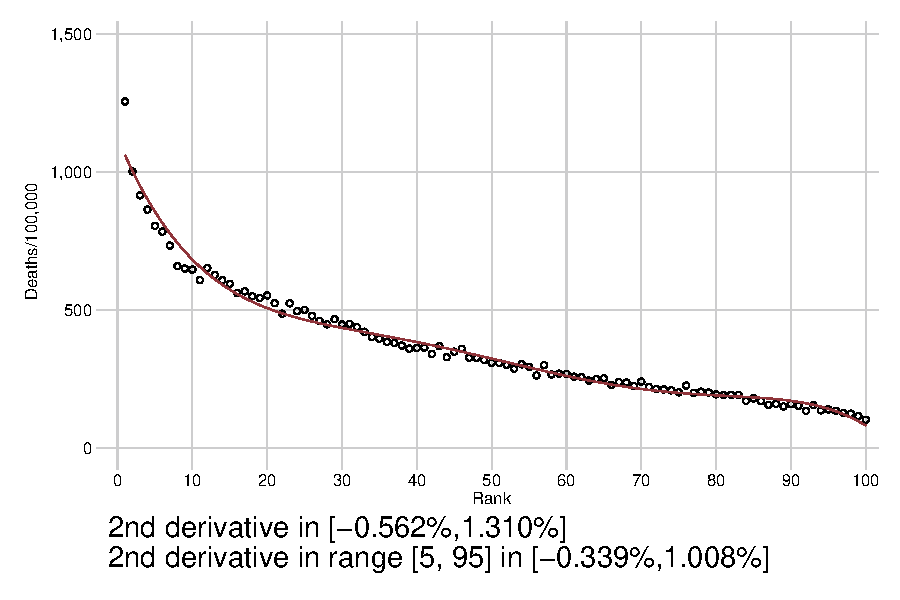
\includegraphics[scale=0.75]{\mortalitypath/polyspline__50_M_2012-2014} %%
  \end{center}                                                            %%
  

  \noindent
  \footnotesize{Figure \ref{fig:mort_poly} presents estimates of
    the conditional expectation function of U.S. mortality given
    income rank, using data from \citet{Chetty2016b}. The CEF is
    fitted using a fifth-order polynomial. The function plots the best
    polynomial fit to the data series, and the circles plot the
    underlying data. The text under the graph shows the range of the
    second derivative, divided by the mean mortality rate in all
    percentiles, across the function's support.}
\end{figure}
